\documentclass[11pt,a4paper]{article}

% Packages
\usepackage[utf8]{inputenc}
\usepackage[T1]{fontenc}
\usepackage{geometry}
\usepackage{graphicx}
\usepackage{hyperref}
\usepackage{enumitem}
\usepackage{booktabs}
\usepackage{longtable}
\usepackage{fancyhdr}
\usepackage{titlesec}
\usepackage{caption}
\usepackage{subcaption}
\usepackage{listings}
\usepackage{xcolor}
\usepackage{amsmath}
\usepackage{tabularx}
\usepackage{array}
\usepackage{float}
\usepackage{tikz}
\usepackage{amssymb}
\usetikzlibrary{shapes.geometric, shapes.misc, arrows.meta, positioning, fit,
                backgrounds, calc, chains, decorations.pathreplacing}

\geometry{margin=2cm,top=2.2cm,bottom=2.2cm}

% ── Colours (for TikZ diagrams) ──────────────────────────────────────────────
\definecolor{clientblue}{RGB}{210,228,255}
\definecolor{gatewaygreen}{RGB}{210,240,220}
\definecolor{svcyellow}{RGB}{255,249,210}
\definecolor{dbgray}{RGB}{225,225,225}
\definecolor{mqorange}{RGB}{255,232,210}
\definecolor{redisred}{RGB}{255,218,218}
\definecolor{bordercolor}{RGB}{80,80,80}

% Header/Footer
\pagestyle{fancy}
\fancyhf{}
\fancyhead[L]{CS7NS6 -- Distributed Systems}
\fancyhead[R]{Exercise 2}
\fancyfoot[C]{\thepage}

% Hyperlink styling
\hypersetup{
    colorlinks=true,
    linkcolor=blue,
    citecolor=blue,
    urlcolor=blue
}

% Code listing style
\lstset{
    basicstyle=\ttfamily\small,
    breaklines=true,
    frame=single,
    backgroundcolor=\color{gray!10},
    keywordstyle=\color{blue},
    commentstyle=\color{green!50!black},
    stringstyle=\color{red!70!black}
}

% ── Table helpers ─────────────────────────────────────────────────────────────
\newcolumntype{L}[1]{>{\raggedright\arraybackslash}p{#1}}
\newcolumntype{C}[1]{>{\centering\arraybackslash}p{#1}}

% ── TikZ node styles ──────────────────────────────────────────────────────────
\tikzset{
  base/.style={draw=bordercolor, line width=0.7pt, align=center,
               font=\footnotesize, minimum height=0.85cm},
  client/.style   = {base, rounded corners=5pt, fill=clientblue,  minimum width=2.8cm},
  gateway/.style  = {base, rounded corners=5pt, fill=gatewaygreen, minimum width=5.2cm, minimum height=1.1cm},
  service/.style  = {base, rounded corners=4pt, fill=svcyellow,   minimum width=2.4cm},
  database/.style = {base, cylinder, shape border rotate=90, aspect=0.3,
                     fill=dbgray, minimum width=1.7cm, minimum height=0.9cm},
  broker/.style   = {base, rounded corners=4pt, fill=mqorange,    minimum width=2.4cm},
  cache/.style    = {base, cylinder, shape border rotate=90, aspect=0.3,
                     fill=redisred, minimum width=1.7cm, minimum height=0.9cm},
  arr/.style      = {-{Stealth[length=5pt]}, line width=0.7pt, color=bordercolor},
  darr/.style     = {-{Stealth[length=5pt]}, line width=0.6pt, dashed, color=bordercolor},
  lifeline/.style = {dashed, line width=0.5pt, color=bordercolor},
  msg/.style      = {-{Stealth[length=4pt]}, line width=0.6pt},
}

\begin{document}

% ============================================================
% TITLE PAGE
% ============================================================
\begin{titlepage}
    \centering
    \vspace*{0.5cm}

    \includegraphics[width=3.5cm]{tcd_logo.png}\\[0.7cm]

    {\Large \textbf{Trinity College Dublin}}\\[0.2cm]
    {\large School of Computer Science and Statistics}\\[1.2cm]

    {\LARGE \textbf{CS7NS6 -- Distributed Systems}}\\[0.4cm]
    {\Large 2025--2026}\\[1cm]

    {\Huge \textbf{Exercise 2:\\Implementing a Globally-accessible\\Distributed Service}}\\[1.5cm]

    {\Large \textbf{Group J}\\[1cm]}

    \begin{tabular}{l l}
        \toprule
        \textbf{Name} & \textbf{Roll Number} \\
        \midrule
        Aditya Kumar Singh & 25340485 \\
        Parth Ashok Deshmukh & 25342469 \\
        Sai Eeshwar Divaakar & 25338829 \\
        Tanmay Ghosh & 25340079 \\
        Saurabh Deshmukh & 25335434 \\
        Sneha Meto & 25337472 \\
        \bottomrule
    \end{tabular}

    \vfill

    {\large \today}

\end{titlepage}

% ============================================================
% TABLE OF CONTENTS
% ============================================================
\newpage
\tableofcontents

\newpage
% ============================================================
% LIST OF ABBREVIATIONS
% ============================================================
\section*{Table of Abbreviations}
\addcontentsline{toc}{section}{Table of Abbreviations}

\begin{table}[H]
\centering\small
\begin{tabularx}{\textwidth}{L{3cm} X}
\toprule
\textbf{Abbreviation} & \textbf{Full Form} \\
\midrule
2PC   & Two-Phase Commit \\
API   & Application Programming Interface \\
CRUD  & Create, Read, Update, Delete \\
DB    & Database \\
DLQ   & Dead Letter Queue \\
DLX   & Dead Letter Exchange \\
Go    & Go Programming Language \\
HA    & High Availability \\
HAProxy & High Availability Proxy \\
HMAC  & Hash-Based Message Authentication Code \\
HTTP  & Hypertext Transfer Protocol \\
JWT   & JSON Web Token \\
LAN   & Local Area Network \\
LRU   & Least Recently Used \\
MD5   & Message Digest Algorithm 5 \\
nginx & Engine-X Web Server / Reverse Proxy \\
p95   & 95th Percentile \\
Py    & Python \\
QPS   & Queries Per Second / Requests Per Second \\
r/s   & Requests Per Second \\
REST  & Representational State Transfer \\
SQL   & Structured Query Language \\
TTL   & Time To Live \\
URL   & Uniform Resource Locator \\
WAL   & Write-Ahead Logging \\
WAN   & Wide Area Network \\
WS    & WebSocket \\
\bottomrule
\end{tabularx}
\caption{Abbreviations used in this report}
\label{tab:abbreviations}
\end{table}

\newpage
% ============================================================
% 1. INTRODUCTION
% ============================================================
\section{Introduction}

This project implements a \textbf{Globally Accessible Distributed Traffic System} allowing road-vehicle drivers to pre-book journeys. No driver may start a journey without a confirmed booking. The system enforces scheduling and road-capacity conflicts, delivers real-time booking notifications via WebSocket connections, and provides sub-second enforcement verification for roadside agents.

The system comprises six independently deployable microservices (User, Journey, Conflict, Notification, Enforcement, Analytics), each with its own PostgreSQL database. Services communicate via synchronous REST  for consistency-critical flows and asynchronous RabbitMQ events for fan-out. Infrastructure includes PostgreSQL WAL  streaming replication, Redis Sentinel for cache high availability , an HAProxy /nginx gateway with rate limiting, and a full multi-node deployment mode where each laptop runs the complete stack.

% ============================================================
% 2. REQUIREMENTS
% ============================================================
\section{Requirements}
\label{sec:requirements}

\subsection{Functional Requirements}

The system addresses the following functional requirements:
 
\begin{enumerate}[label=\textbf{FR\arabic*}]
    \item \textbf{User Registration and Authentication:} Drivers and enforcement agents can register accounts and authenticate via JWT (JSON Web Token) tokens. Passwords are hashed with bcrypt. Separate "DRIVER" and "ENFORCEMENT\_AGENT" roles are supported. Vehicle registration is linked to user accounts.
    \item \textbf{Journey Booking:} Drivers can create journey bookings specifying origin, destination (with coordinates), departure time, estimated duration, and vehicle registration. Bookings are confirmed only after passing conflict checks. The system returns "CONFIRMED" or "REJECTED" with a reason.
    \item \textbf{Conflict Detection:} The system checks for three types of conflicts before confirming a booking: driver overlap (same driver has an overlapping confirmed journey), vehicle overlap (same vehicle already booked), and road-segment capacity (grid cell at maximum capacity for the time slot).
    \item \textbf{Journey Cancellation:} Drivers can cancel their own bookings. Cancellation releases reserved road capacity, removes enforcement cache entries, and notifies all downstream services via event fan-out.
    \item \textbf{Real-time Notifications:} Drivers receive push notifications via WebSocket for booking confirmations, rejections, and cancellations. A notification history endpoint provides the last 50 entries with a 7-day TTL (Time To Live).
    \item \textbf{Enforcement Verification:} Enforcement agents can verify whether a vehicle or driver holds an active booking by querying by vehicle plate or driving licence number with sub-second response times.
    \item \textbf{Analytics and Monitoring:} The system records journey events, provides real-time statistics, hourly aggregated reports, and an aggregated health view of all services.
    \item \textbf{Points System:} Each confirmed journey earns the driver points based on distance and duration, tracked via a pessimistically locked points ledger.
    \item \textbf{Idempotent Retries:} Clients supply an "Idempotency-Key" header; duplicate booking requests return the cached result without re-running the saga.
\end{enumerate}
 
\subsection{Non-Functional Requirements}
\label{sec:nfr}

Targets are motivated by a "write-heavy, geographically distributed" load profile. At 1M active drivers nationally, assuming 30\% book during a 30-minute morning peak, arrival rate is $\approx$167 bookings/s; the two-node demo targets 50 bookings/s per node. Enforcement checks are high-frequency reads ($<200$\,ms) motivating the Redis-first lookup design.

\begin{table}[H]
\centering\small
\begin{tabularx}{\textwidth}{L{3.2cm} L{4.4cm} X}
  \toprule
  \textbf{Property} & \textbf{Target} & \textbf{Rationale / Mechanism} \\
  \midrule
  Availability & $\geq 99.5\%$ under a single node failure & Active-active
        deployment: clients transparently fail over to a surviving node
        through the browser's "resilientFetch" layer. \\
  Booking latency & $<400\,$ms at p95 (95th percentile) under normal load & End-to-end saga (journey row $\to$ conflict check $\to$ outbox) benchmarks at 100--250\,ms on the slim stack. \\
  Enforcement latency & $<200\,$ms hard limit (cache hit $<20\,$ms p95) & Redis-first lookup with a journey-service fallback path. \\
  Consistency & Strong per-slot (no double booking) & "SERIALIZABLE"
        transaction with "SELECT FOR UPDATE" inside the conflict
        service. \\
  Eventual consistency & Cross-service state converges after a partition
        heals & Transactional outbox $+$ at-least-once RabbitMQ delivery,
        idempotent consumers. \\
  Durability & No confirmed booking is ever lost & Event stored in the same
        DB transaction as the journey row; background drainer replays to
        RabbitMQ after broker recovery. \\
  Fault Tolerance & System degrades, does not crash & Transactional outbox pattern, circuit breakers, Redis Sentinel, and Postgres streaming replication. When the conflict service is unreachable, the circuit breaker opens and bookings fail fast rather than hanging. When infrastructure peers are down, the system enters "LOCAL\_ONLY" mode. \\
  Partition tolerance & System degrades gracefully & Partition manager
        per service (CONNECTED $\to$ SUSPECTED $\to$ PARTITIONED $\to$
        MERGING). Circuit breaker fails fast on dependency outage. \\
  Scalability & Independent service scaling & The microservices architecture allows independent scaling of services. Read/write separation via PostgreSQL replicas offloads read traffic. \\
  Idempotency & No duplicate side effects & Duplicate booking requests (same idempotency key) return cached results. Message consumers deduplicate via Redis "SETNX" on message IDs. \\
  Observability & All cross-service calls traceable & "X-Request-ID"
        propagated; "X-Partition-Status" and
        "X-Cache-Stale" headers exposed on responses. \\
  \bottomrule
\end{tabularx}
\caption{Non-functional requirements}
\label{tab:nfr}
\end{table}

\subsection{Failure Model}

We adopt a \textbf{crash-recovery} failure model with asynchronous network. Services may crash and restart at any time; all durable state lives in PostgreSQL, RabbitMQ or Redis. Messages between services may be delayed, duplicated or lost. We assume a trusted internal network between services, so Byzantine faults are out of scope. Correlated failures are mitigated by running the full stack on each participating node so that losing one laptop does not take the system down.

% ============================================================
% 3. SPECIFICATION
% ============================================================
\section{Specification}
\label{sec:specification}
 
\subsection{System Services}
 
The system is composed of six independent microservices, each with its own Postgres database:
 
\begin{table}[H]
\centering\small
\begin{tabularx}{\textwidth}{L{2.7cm} L{1.4cm} L{2.6cm} X}
  \toprule
  \textbf{Service} & \textbf{Lang / Port} & \textbf{Data store} & \textbf{Responsibility} \\
  \midrule
  User          & Python / 8001 & Postgres "users\_db" + replica &
      Registration, login (JWT), vehicle CRUD. Publishes
      "user.registered". Routes reads to replica, writes to primary. \\
  Journey       & Python / 8002 & Postgres "journeys\_db" + replica &
      Booking saga orchestration, idempotency, outbox drainer, circuit
      breaker, lifecycle scheduler, partition detector, 2PC (Two-Phase Commit) coordinator,
      peer health model. \\
  Conflict      & Go / 8003 & Postgres "conflicts\_db" + replica &
      Atomic capacity check ("SERIALIZABLE" + "SELECT FOR UPDATE"),
      grid-cell road model ($\approx$ 0.01\textdegree, approximately 1\,km per cell, 30-minute time slots), REST slot replication to peer nodes, idempotent
      cancellation consumer. \\
  Notification  & Go / 8004 & Redis &
      WebSocket push, consumer deduplication via Redis "SETNX",
      notification history (7-day TTL, 50 entries/user), DLQ (Dead Letter Queue),
      auto-reconnect. \\
  Enforcement   & Python / 8005 & Redis + journey API &
      Redis-first lookup; licence$\to$user id cache (24\,h TTL);
      event-driven invalidation; "X-Cache-Stale" header on
      partition. \\
  Analytics     & Go / 8006 & Postgres "analytics\_db" + replica + Redis &
      Dual-write counters, hourly roll-up goroutine, replica-lag endpoint,
      aggregated service health. \\
  \bottomrule
\end{tabularx}
\caption{Service inventory}
\label{tab:services}
\end{table}

\subsection{Service APIs}

All external traffic enters through HAProxy, which forwards requests to two nginx instances in full-stack mode or a single nginx instance in slim mode. We implemented an API Gateway pattern using Nginx as the single entry point for all client traffic. This design decouples the frontend from the internal service topology and allows us to enforce global security policies, such as rate limiting (e.g., 5 requests/sec for auth endpoints). Nginx applies three rate-limit zones: auth (5 r/s, burst 10), booking (10 r/s, burst 20), and general (30 r/s, burst 10–20). It also handles request routing based on URL prefixes. Table~\ref{tab:api} lists all public API endpoints.

\begin{table}[H]
\centering
\scriptsize
\setlength{\tabcolsep}{3pt}
\begin{tabularx}{\textwidth}{L{1.6cm} @{\hspace{6pt}} L{1.1cm} @{\hspace{6pt}} L{6.2cm} @{\hspace{6pt}} X}
  \toprule
  \textbf{Service} & \textbf{Method} & \textbf{Path} & \textbf{Description} \\
  \midrule
 
  %% ── User Service ──────────────────────────────────────────────────
  User (Python)
    & GET    & \texttt{/api/users/me}                                       & Current user's profile \\
    & GET    & \texttt{/api/users/license/\{license\_number\}}              & Look up user by licence number \\
    & GET    & \texttt{/api/users/vehicles}                                 & List current user's vehicles \\
    & GET    & \texttt{/api/users/vehicles/verify/\{registration\}}         & Verify vehicle ownership \\
    & POST   & \texttt{/api/users/register}                                 & Register a driver account \\
    & POST   & \texttt{/api/users/register/agent}                           & Register an enforcement agent account \\
    & POST   & \texttt{/api/users/login}                                    & Login, returns JWT token \\
    & POST   & \texttt{/api/users/vehicles}                                 & Register a vehicle \\
    & DELETE & \texttt{/api/users/vehicles/\{vehicle\_id\}}                 & Remove a vehicle \\
  \midrule
 
  %% ── Journey Service ───────────────────────────────────────────────
  Journey (Python)
    & GET    & \texttt{/api/journeys/}                                      & List current user's journeys \\
    & GET    & \texttt{/api/journeys/all}                                   & Admin: all journeys across all users \\
    & GET    & \texttt{/api/journeys/\{journey\_id\}}                       & Get a specific journey \\
    & GET    & \texttt{/api/journeys/points/balance}                        & Current user's points balance \\
    & GET    & \texttt{/api/journeys/points/history}                        & Points transaction history \\
    & GET    & \texttt{/api/journeys/vehicle/\{vehicle\_reg\}/active}       & Active journeys for a vehicle \\
    & GET    & \texttt{/api/journeys/user/\{user\_id\}/active}              & Active journeys for a user \\
    & POST   & \texttt{/api/journeys/} (\texttt{?mode=2pc})                 & Book a journey (saga / Two-Phase Commit) \\
    & POST   & \texttt{/api/journeys/points/spend}                          & Spend points (\texttt{?amount=}) \\
    & DELETE & \texttt{/api/journeys/\{journey\_id\}}                       & Cancel a journey \\
  \midrule
 
  %% ── Conflict Service ──────────────────────────────────────────────
  Conflict (Go)
    & GET    & \texttt{/api/routes}                                         & List all road routes \\
    & GET    & \texttt{/api/conflicts/routes}                               & Same as above (alternate nginx prefix) \\
    & POST   & \texttt{/api/conflicts/check}                                & Check capacity conflicts before booking \\
    & POST   & \texttt{/api/conflicts/cancel/\{journey\_id\}}               & Cancel a booking slot (frees capacity) \\
  \midrule
 
  %% ── Enforcement Service ───────────────────────────────────────────
  Enforcement (Python)
    & GET    & \texttt{/api/enforcement/verify/vehicle/\{reg\}}    & Verify vehicle has active booking (agent only) \\
    & GET    & \texttt{/api/enforcement/verify/license/\{lic\_no\}} & Verify driver by licence number (agent only) \\
  \midrule
 
  %% ── Notification Service ──────────────────────────────────────────
  Notification (Go)
    & GET    & \texttt{/api/notifications/}                                 & Get notifications (\texttt{?token=}, \texttt{?limit=}) \\
    & WS     & \texttt{/ws/notifications/}                                  & WebSocket stream of real-time notifications (\texttt{?token=}) \\
  \midrule
 
  %% ── Analytics Service ─────────────────────────────────────────────
  Analytics (Go)
    & GET    & \texttt{/api/analytics/stats}                                & System-wide booking stats \\
    & GET    & \texttt{/api/analytics/events}                               & Event history (\texttt{?event\_type=}, \texttt{?limit=}, \texttt{?offset=}) \\
    & GET    & \texttt{/api/analytics/hourly}                               & Hourly booking stats (\texttt{?limit=}, max 168h) \\
    & GET    & \texttt{/api/analytics/replica-lag}                          & PostgreSQL replication lag (\texttt{pg\_stat\_replication}) \\
    & GET    & \texttt{/api/analytics/health/services}                      & Aggregate health check of all 6 services \\
  \midrule
 
  %% ── Health / Admin (cross-service) ────────────────────────────────
  All services
    & GET    & \texttt{/health}                                             & Health check (503 when node simulated-failed) \\
    & GET    & \texttt{/health/partitions}                                  & Partition status of dependencies \\
    & GET    & \texttt{/health/nodes}                                       & Per-peer ALIVE / SUSPECT / DEAD status \\
    & GET    & \texttt{/admin/logs}                                         & Recent log entries (ring buffer) \\
    & GET    & \texttt{/admin/simulate/status}                              & Current simulation state \\
    & POST   & \texttt{/admin/simulate/fail}                                & Simulate node crash (cascades to user-service) \\
    & POST   & \texttt{/admin/simulate/recover}                             & Recover from simulated failure \\
    & POST   & \texttt{/admin/peers/register}                               & Register a remote peer to monitor \\
    & POST   & \texttt{/admin/recovery/drain-outbox}                        & Force-drain unpublished outbox events \\
    & POST   & \texttt{/admin/recovery/rebuild-enforcement-cache}           & Rebuild enforcement Redis cache from DB \\
    & POST   & \texttt{/admin/2pc/demo}                                     & Info on triggering 2PC demo \\
    & DELETE & \texttt{/admin/peers/\{name\}}                               & Unregister a peer \\
  \bottomrule
\end{tabularx}
\caption{Full API surface across all six microservices}
\label{tab:api}
\end{table}

\subsection{Internal APIs and Events}
\label{sec:internal-apis}

Two additional interfaces exist purely between services and are not exposed through the public gateway:

\begin{itemize}
  \item \textbf{REST (south-bound, cross-node replication).}
    "POST /api/conflicts/check" (Journey $\to$ Conflict; reserves
    a slot inside a serialisable transaction) and
    "POST /api/conflicts/cancel/\{id\}" (compensating call used
    by the 2PC coordinator). Cross-node replication uses the
    "/internal/slots/*" family on the Conflict Service
    ("replicate", "cancel", "active") and the
    "/internal/users/*" family on the User Service
    ("lock", "replicate", "snapshot") described in
    Sections~\ref{sec:replication} and the User Service design.
  \item \textbf{RabbitMQ topic exchange "journey\_events".}
    Routing keys: "user.registered", "journey.confirmed",
    "journey.rejected", "journey.cancelled",
    "journey.completed". Each consumer binds its own durable
    queue and is wired to a per-consumer dead-letter exchange
    ("{queue}.dlx") with a 24-hour TTL on the DLQ so poison
    messages are retained for inspection without blocking the main
    queue.
\end{itemize}

\subsection{Fault Behaviour}
 
The system is designed to handle the following fault scenarios. Table~\ref{tab:faults} captures how the system responds to each important failure class.

\begin{table}[H]
\centering\footnotesize
\begin{tabularx}{\textwidth}{L{2.8cm} X L{3.8cm}}
  \toprule
  \textbf{Fault} & \textbf{System behaviour} & \textbf{Guarantee} \\
  \midrule
  Journey service crash & Outbox drainer resumes on restart; browser \texttt{resilientFetch} retries peer. & No confirmed booking lost; idempotent retries. \\
  Conflict service crash & \texttt{conflict\_client.py} tries local then each \texttt{PEER\_CONFLICT\_URLS} entry; per-URL circuit breakers open after 3 failures. & Booking fails only when all known endpoints exhausted. \\
  RabbitMQ outage & Outbox row persisted in same DB tx; drainer replays on reconnect. & At-least-once delivery; downstream eventual consistency. \\
  Redis primary loss & Sentinel (quorum 2) promotes replica; services auto-reconnect. & Cache availability, bounded staleness. \\
  Postgres replica lag & Reads fall back to primary; lag visible at \texttt{/api/analytics/replica-lag}. & Read availability. \\
  Network partition & Replication back-fills after merge via 5-min re-sync goroutine. & No local double bookings; eventual global convergence. \\
  Full-node kill & Journey+user set \texttt{\_node\_failed=True}; all routes return 503. Browser fails over transparently. & Session preserved via shared JWT secret; peer-list in localStorage. \\
  Peer node failure & ALIVE→SUSPECT (3 missed pings) →DEAD (6 missed). $<$50\% alive → \texttt{LOCAL\_ONLY} mode. & Graceful degradation. \\
  Message redelivery & Redis \texttt{SETNX} dedup on message ID (24\,h TTL) in all consumers. & Effectively-exactly-once processing. \\
  \textbf{Known gaps} & No saga compensation retry; no token blacklist; enforcement cache cold on boot; RabbitMQ cluster unreliable on single host. & --- \\
  \bottomrule
\end{tabularx}
\caption{Fault-handling matrix}
\label{tab:faults}
\end{table}

\subsection{Limitations and Unaddressed Requirements}
\label{sec:limitations}

The following limitations are known and documented as honest trade-offs rather than silent gaps:

\begin{itemize}
    \item \textbf{Saga compensating transactions:} If the Conflict Service is permanently unreachable during a booking, the saga rejects the booking with no automatic retry or compensation loop.
    \item \textbf{Audit HMAC chain:} The \texttt{event\_logs} table records a full event history with timestamps, but the planned cryptographic integrity chain (HMAC over sequential rows) was not completed.
    \item \textbf{WebSocket registry:} The Notification Service holds its WebSocket connection registry in process memory only; a service restart drops all live connections and clients must reconnect.
    \item \textbf{Enforcement cache cold start:} After a restart, the first enforcement request always misses the Redis cache and pays the fallback-REST cost; there is no cache warming on boot.
    \item \textbf{Token blacklisting:} Revoked JWT tokens remain valid until their natural expiry; no deny-list is maintained on logout.
    \item \textbf{RabbitMQ clustering:} A 3-node RabbitMQ cluster is configured, but Erlang distribution is unreliable on a single Docker host. The single-node deployment demonstrates all messaging semantics.
    \item \textbf{Distributed tracing visualisation:} Correlation IDs (\texttt{X-Request-ID}) propagate across all services, but no span visualisation tool (Jaeger, Zipkin) is integrated.
\end{itemize}

% ============================================================
% 4. ARCHITECTURE AND DESIGN
% ============================================================
\section{Architecture and Design}
\label{sec:architecture}
 
\subsection{System Architecture}
 \begin{figure}[H]
    \centering
    \includegraphics[width=1\textwidth]{newarch.png}
    \caption{System architecture.}
\end{figure}
Six microservices, each owning its own database. HAProxy (full-stack) load-balances across two nginx instances; slim mode uses a single nginx on port 8080. Nginx rate-limits (auth 5\,r/s, booking 10\,r/s, general 30\,r/s) and routes by URL prefix using per-request DNS re-resolution (\texttt{set \$svc; proxy\_pass http://\$svc;}) to avoid stale-IP routing after container recreation. Services communicate synchronously via REST (Journey→Conflict for saga) and asynchronously via RabbitMQ topic exchange \texttt{journey\_events}. In multi-node mode, the entire stack runs on every laptop; nodes discover each other via \texttt{PEER\_CONFLICT\_URLS}/\texttt{PEER\_USER\_URLS} env vars and \texttt{POST /admin/peers/register}.

\begin{figure}[H]
\centering
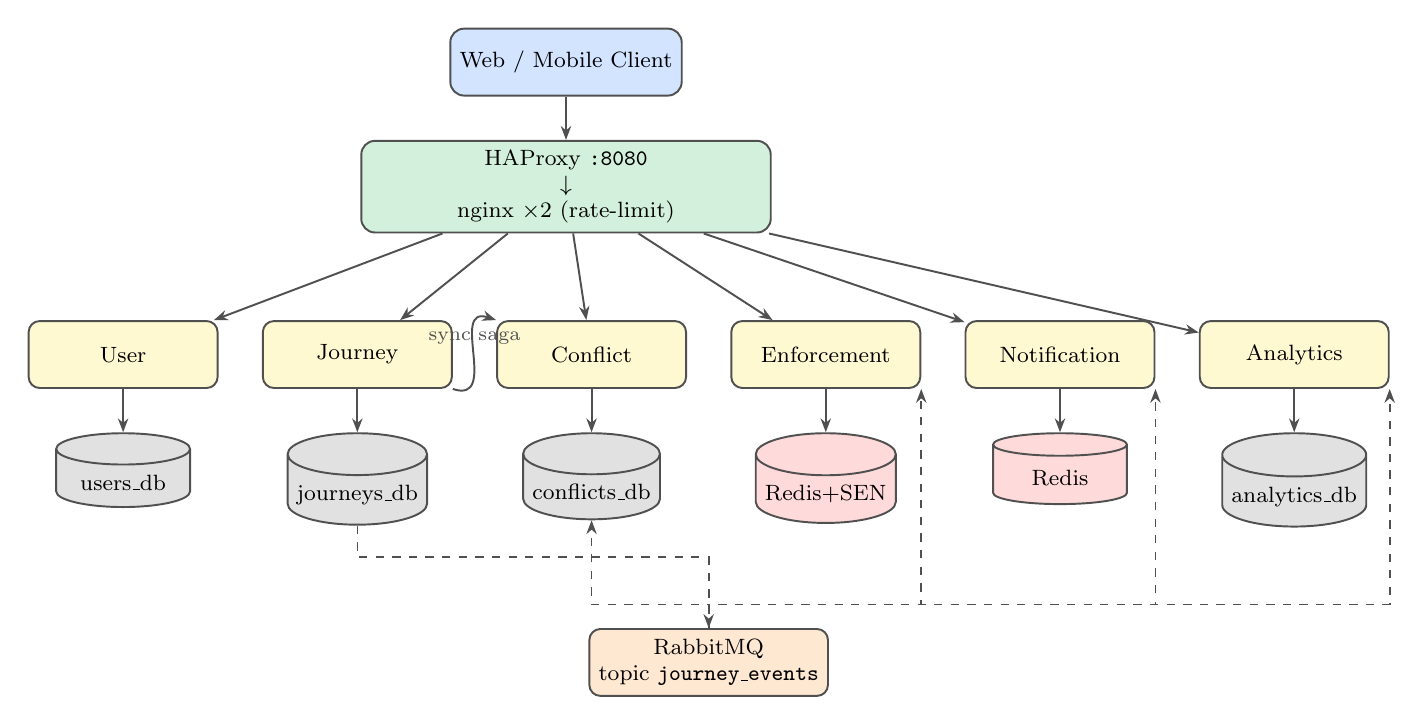
\begin{tikzpicture}[node distance=0.55cm and 0.55cm]
  \node[client] (client) {Web / Mobile Client};
  \node[gateway, below=of client] (gw)
       {HAProxy \texttt{:8080} \\ $\downarrow$ \\ nginx $\times 2$ (rate-limit)};
  \node[service, below left=1.1cm and 1.8cm of gw] (user)  {User};
  \node[service, right=of user]                     (jrny)  {Journey};
  \node[service, right=of jrny]                     (cnf)   {Conflict};
  \node[service, right=of cnf]                      (enf)   {Enforcement};
  \node[service, right=of enf]                      (notif) {Notification};
  \node[service, right=of notif]                    (anl)   {Analytics};
  \node[database, below=of user]  (udb)  {users\_db};
  \node[database, below=of jrny]  (jdb)  {journeys\_db};
  \node[database, below=of cnf]   (cdb)  {conflicts\_db};
  \node[cache,    below=of enf]   (rds)  {Redis+SEN};
  \node[cache,    below=of notif] (nrd)  {Redis};
  \node[database, below=of anl]   (adb)  {analytics\_db};

  % Centre RabbitMQ below the database row, midpoint of all services
  \path (udb.south) -- (adb.south) coordinate[midway] (dbmid);
  \node[broker, below=1.4cm of dbmid] (mq) {RabbitMQ \\ topic \texttt{journey\_events}};

  \draw[arr] (client)--(gw);
  \foreach \s in {user,jrny,cnf,enf,notif,anl} \draw[arr] (gw)--(\s);
  \draw[arr] (user)--(udb);
  \draw[arr] (jrny)--(jdb);
  \draw[arr] (cnf)--(cdb);
  \draw[arr] (anl)--(adb);
  \draw[arr] (enf)--(rds);
  \draw[arr] (notif)--(nrd);
  \draw[arr] (jrny.south east) .. controls +(0.6,-0.2) and +(-0.6,0.2) .. (cnf.north west)
        node[midway,above,font=\scriptsize]{sync saga};
  \draw[darr] (jdb.south) -- ++(0,-0.4) -| (mq);
  \draw[darr] (mq.north) -- ++(0,0.3) -| (notif.south east);
  \draw[darr] (mq.north) -- ++(0,0.3) -| (enf.south east);
  \draw[darr] (mq.north) -- ++(0,0.3) -| (anl.south east);
  \draw[darr] (mq.north) -- ++(0,0.3) -| (cdb.south);
\end{tikzpicture}
\caption{High-level runtime topology. Solid arrows are synchronous REST;
dashed arrows are asynchronous RabbitMQ events. Each service owns its
database; Redis+Sentinel backs enforcement, notification and analytics.}
\label{fig:architecture}
\end{figure}

 
\subsection{Infrastructure and Middleware}

Services are implemented in Python (User, Journey, Enforcement) and Go (Conflict, Notification, Analytics). All Python services share modules in "shared/": "circuit\_breaker.py" (CLOSED / OPEN / HALF\_OPEN), "partition.py" (dependency probes every 5\,s), "rabbitmq.py" (durable publish/consume, DLX wiring), and "tracing.py" ("X-Request-ID" propagation). Go services use equivalent hand-written packages.

Infrastructure (full-stack): 26 containers — 6 services, 8 Postgres (4 primary+replica pairs), 2 Redis instances, 3 Sentinel instances, 3 RabbitMQ nodes, 2 nginx, 1 HAProxy, 1 frontend. Slim profile: 12 containers.

\textbf{Middleware choices:} \textbf{RabbitMQ} (topic exchange "journey\_events") decouples booking confirmation from downstream fan-out; consumers (Notification, Analytics, Enforcement) process at their own pace with DLQ on failure. Dead-letter exchanges (DLX) route unprocessable messages with 24-hour TTL. \textbf{Redis} provides sub-millisecond reads for enforcement caching and deduplication keys; Sentinel (quorum 2) auto-promotes on primary failure. \textbf{HAProxy} load-balances across two nginx instances (full-stack); slim mode uses a single nginx. \textbf{PostgreSQL} WAL streaming replication separates reads (replica) from writes (primary); "SERIALIZABLE" isolation is used only in the Conflict Service to avoid locking overhead on ordinary CRUD (Create, Read, Update, Delete) paths.

\subsection{Individual Service Designs}
 
Each team member was responsible for the design of one or more services. The following subsections describe the most significant service each member contributed.
 
\subsubsection{User Service: Parth Deshmukh}
 
The User Service provides stateless JWT-based authentication and serves as the entry point for driver and enforcement agent registration. It routes read queries to a Postgres streaming replica and write queries to the primary, implementing read/write separation at the application level via a "Session.get\_bind()" override at the SQLAlchemy level.

\textbf{Distributed lock (Redlock-style, 2-phase):} Before inserting a new user, the registering node (1) acquires "user\_email\_lock:\{email\}" via Redis "SETNX" with a 15\,s TTL on its local Redis, (2) POSTs "/internal/users/lock" to every peer, each peer checks email uniqueness and acquires its own SETNX, and (3) if any peer rejects (email already exists or lock contention), the requesting node rolls back all acquired locks and returns HTTP 409. This prevents split-brain registrations where two nodes simultaneously accept the same email address.

\textbf{Consistent-hash sharding:} Every email is hashed as "shard\_id = MD5(email) \% num\_nodes". The node where "shard\_id == 0" is the "home shard", the authoritative writer for that user. All nodes still hold all data (active-active replication), so sharding governs write authority and observability, not data isolation.

On successful registration, the service publishes a "user.registered" event to RabbitMQ, then asynchronously replicates the new user record to every peer via "POST /internal/users/replicate". A background loop additionally pulls a full user/vehicle snapshot from each peer on startup and every 5 minutes (catch-up sync), filling any gap that accumulated during downtime. JWTs are signed with a shared secret across nodes, which allows the browser to re-use a session on the failover peer without a re-login.

During a simulated node kill, the service installs an HTTP middleware that returns 503 for every path except "/health", "/admin/simulate/fail" and "/admin/simulate/recover", so from a peer's point of view the entire user-facing surface of the node disappears at once.
 
\subsubsection{Journey Service: Tanmay Ghosh}
 
The Journey Service is the most architecturally complex service in the system, serving as the saga orchestrator. Its design centres on several distributed systems patterns:
 
The \textbf{transactional outbox} ensures that journey state changes and their corresponding events are written atomically in a single database transaction to the "outbox\_events" table. A background task polls this table every 2 seconds (filtering on "published = false") and drains unpublished events to RabbitMQ, guaranteeing at-least-once delivery even if the broker is temporarily unavailable. Coupling the domain write to the event write eliminates the dual-write problem ("wrote to DB, crashed before publish") without needing a distributed transaction.
 
The \textbf{circuit breaker} wraps the synchronous REST call to the Conflict Service. It tracks consecutive failures and, after a configurable threshold (default: 3), opens the circuit so that subsequent booking requests fail immediately rather than accumulating timeouts.
 
The \textbf{partition detection} module probes Postgres, RabbitMQ, and the Conflict Service every 5 seconds, transitioning through "CONNECTED" $\rightarrow$ "SUSPECTED" $\rightarrow$ "PARTITIONED" $\rightarrow$ "MERGING" states. The current state is attached to every HTTP response via the "X-Partition-Status" header.
 
The \textbf{lifecycle scheduler} runs as a background task, transitioning journeys from "CONFIRMED" to "IN\_PROGRESS" (at departure time) and from "IN\_PROGRESS" to "COMPLETED" (at estimated arrival time).

Booking requests optionally carry an "idempotency\_key" field whose value is persisted in an "idempotency\_records" table. If a second request arrives with the same key, the original journey is returned without re-executing the saga, giving exactly-once booking semantics from the client's point of view.

The \textbf{resilient conflict client} ("conflict\_client.py") adds service-level failover: it tries the local conflict-service first, then each URL in "PEER\_CONFLICT\_URLS" in order. Per-URL circuit breakers (CLOSED/OPEN/HALF\_OPEN) wrap each endpoint independently, so a crashed local conflict-service opens only its own breaker while the peer endpoint remains available. For 2PC cancellations, the client prefers the same peer URL that executed the PREPARE phase to avoid phantom-slot leaks.
\subsubsection{Conflict Detection Service: Sneha Meto}
 
The Conflict Service is implemented in Go and is responsible for ensuring that no two bookings conflict on driver schedule, vehicle allocation, or road-segment capacity.
 
Road-segment capacity is modelled using a geographic grid-cell approach with a resolution of 0.01\textdegree{} (approximately 1\,km per cell at 53$^\circ$N). Each cell maintains a count of bookings per 30-minute time slot. This design \emph{exploits spatial locality}: the lock scope of a booking is bounded to the grid cells its route actually traverses, so two bookings on non-overlapping road segments never contend. For predefined routes the actual road waypoints are used to walk only the cells the road passes through, avoiding false conflicts between routes that are geographically close but physically separate.

\textbf{Consistent-hash sharding:} Routes are assigned to shard nodes as "shard = MD5(route\_id) \% num\_nodes". The node where "shard == 0" is PRIMARY for write authority on that route's bookings. This is logged on every conflict check so the activity feed can show which node is acting as primary vs replica for each route.
 
The core design decision is the use of a single "SERIALIZABLE" transaction with "SELECT FOR UPDATE" for the entire check-and-reserve operation. This guarantees that two concurrent booking requests targeting the same cell and time slot cannot both succeed when only one slot remains. The three checks, driver overlap, vehicle overlap, and road capacity, all execute within this single transaction. Two concurrent bookings for the same slot can never both pass: the second transaction either deadlocks and retries or sees the first reservation committed.
 
The service also consumes "journey.cancelled" events from RabbitMQ to release reserved capacity. The consumer is idempotent: redelivered cancellation events find the slot already marked "is\_active = false" and are acknowledged silently without triggering errors or DLQ routing.

The service also implements active-active slot replication (Section~\ref{sec:replication}), making it the only service that holds shared state across nodes.
 
\subsubsection{Notification Service: Aditya Kumar Singh}
 
The Notification Service is implemented in Go and provides real-time push delivery to drivers via WebSocket connections. When a journey event is received from RabbitMQ, the service looks up the target user's in-memory WebSocket connection registry (a "map[user\_id][]*websocket.Conn" guarded by a "sync.RWMutex") and fans out to all open tabs simultaneously. Dead connections are cleaned up lazily on the next write error.

Notification history is stored per user in Redis as a capped list with a 7-day TTL and a maximum of 50 entries per user. Each write is a pipelined "LPUSH" + "LTRIM 0 49" + "EXPIRE 7d", so the newest notification is always at index 0 and old entries fall off the tail automatically. Drivers retrieve missed notifications via the "GET /api/notifications/" REST endpoint.

Consumer deduplication is keyed on \texttt{notif:processed:\{MessageId\}} when the broker did not assign a "MessageId". On each delivery the consumer first issues "EXISTS" on the key; if present, the message is acknowledged and skipped without invoking the handler. On the non-duplicate path the handler runs and the consumer then calls "SET key 1 EX 86400" to mark the message processed for 24\,hours. This turns the at-least-once delivery guarantee of RabbitMQ into an effectively-exactly-once push to the user. On broker disconnect the consumer reconnects with a fixed 3-second retry interval (up to 10 attempts on initial connect). Unprocessable messages are "Nack"'d without requeue and routed through the shared fanout DLX "journey\_events\_dlx" into the "dead\_letter\_queue"; a 24-hour "x-message-ttl" is additionally set on the main "notification\_events" queue so stuck messages eventually expire into the DLX rather than blocking the consumer.

A known limitation is that the WebSocket connection registry is held entirely in process memory. If the Notification Service restarts, all active WebSocket connections are lost and clients must reconnect; the Redis-backed history list ensures no notification is lost, only the live push.
 
\subsubsection{Enforcement Service: Saurabh Deshmukh}
 
The \textbf{Enforcement Service} (Python, port 8005) is designed for roadside verification where sub-second response time is critical. It follows a Redis-first lookup pattern: when an enforcement agent queries by vehicle plate, the service checks "active\_journey:vehicle:\{plate\}" in Redis. On a hit, the cached journey data is returned immediately (measured $<20$\,ms p95). On a miss, the service falls back to querying the Journey Service HTTP API, populates the cache and returns.

\textbf{Cache replacement strategy:} Entries are TTL-evicted; the expiry is set to "(estimated-arrival-time: now) + 3600\,s" so the cache entry slightly outlasts the journey window. For event-driven eviction, the RabbitMQ consumer deletes entries immediately on "journey.cancelled" and "journey.completed". Licence-to-user-ID mappings use a fixed 24-hour TTL. There is no LRU eviction at the application level; Redis handles memory pressure via its own eviction policy ("allkeys-lru" in the slim stack).

When partition detection indicates the Journey Service is unreachable, responses continue from the cache with response headers "X-Data-Staleness: STALE" and "X-Partition-Status: journey-service: PARTITIONED" to alert the agent. A known limitation is that the cache is cold on startup and there is no cache warming on boot.
 
\subsubsection{Analytics \& Monitoring Service: Sai Eeshwar Divaakar}
 
The \textbf{Analytics Service} (Go, port 8006) records every journey and user event to both Postgres ("event\_logs" table, immutable audit trail) and Redis atomically ("analytics:daily:\{YYYY-MM-DD\}" hash counters, 48-hour TTL). Consumer deduplication via Redis "SETNX" on message IDs prevents double-counting on redelivery. The "/api/analytics/stats" endpoint reads Redis for real-time counters and Postgres for all-time totals, giving the frontend both an up-to-the-second view and a historical one.

An hourly rollup goroutine fires every 60 minutes and aggregates the preceding hour's "event\_logs" rows into the "hourly\_stats" table (columns: "hour", "total\_bookings", "confirmed", "rejected", "cancelled"). The first run on startup backfills the previous hour so there is no data gap after a restart.

The service also serves as the system-wide monitoring hub. It exposes Postgres replica lag via "pg\_stat\_replication" at "/api/analytics/replica-lag", providing live proof that WAL streaming replication is active across all four service databases. The aggregated health endpoint ("/api/analytics/health/services") probes all six services' "/health" endpoints in parallel and returns a combined report with response times, serving as a single point of observability for the entire system.




% ============================================================
% 5. IMPLEMENTATION
% ============================================================
\section{Implementation}
\label{sec:implementation}

\subsection{Happy-Path Booking Saga}

The primary operational flow is the journey booking saga. Figure~\ref{fig:saga} shows the sequence of a successful booking: the synchronous portion lasts until the saga either confirms or rejects; the asynchronous fan-out runs entirely off the critical path through RabbitMQ.

\begin{figure}[H]
\centering
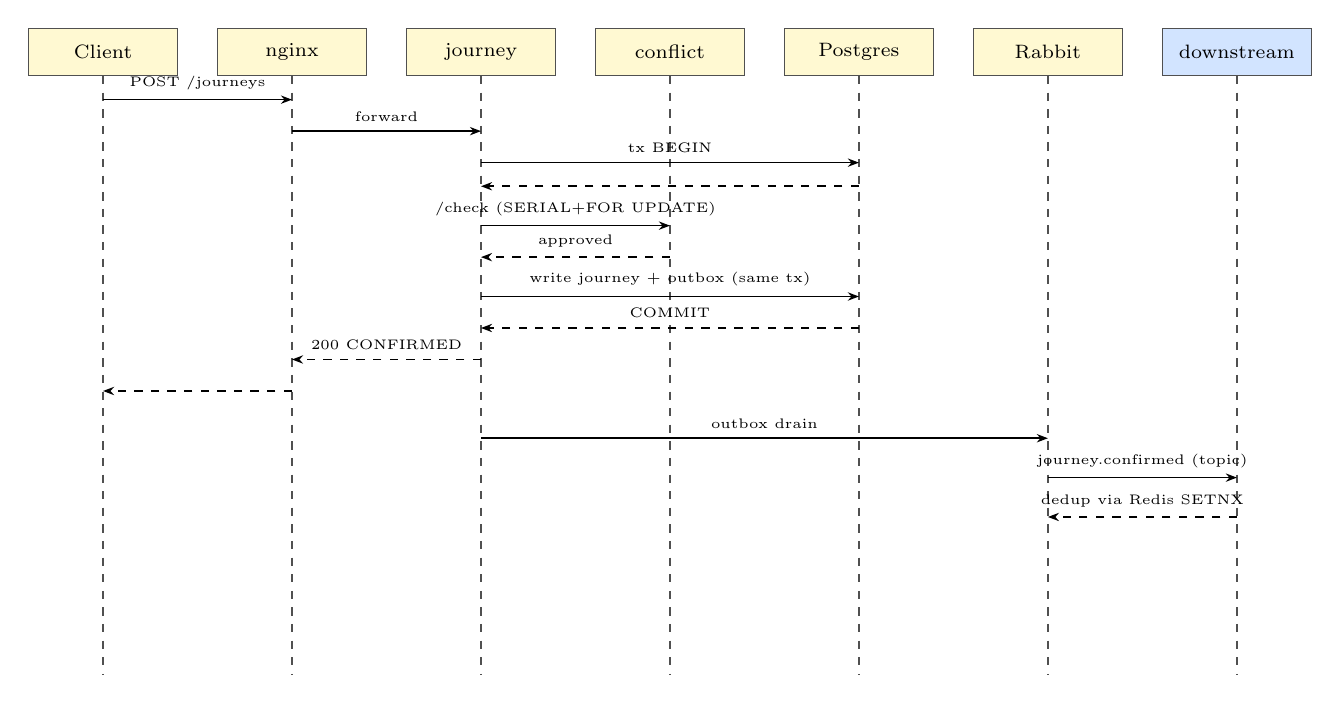
\begin{tikzpicture}[
  actor/.style={draw=bordercolor, fill=svcyellow, minimum width=1.9cm,
                minimum height=0.6cm, font=\scriptsize, align=center},
  font=\scriptsize,
  node distance=0.2cm
]
  \node[actor] (c)   at (0,0)   {Client};
  \node[actor] (gw)  at (2.4,0) {nginx};
  \node[actor] (j)   at (4.8,0) {journey};
  \node[actor] (cf)  at (7.2,0) {conflict};
  \node[actor] (db)  at (9.6,0) {Postgres};
  \node[actor] (mq)  at (12,0)  {Rabbit};
  \node[actor,fill=clientblue] (dn) at (14.4,0) {downstream};

  \foreach \n in {c,gw,j,cf,db,mq,dn}
    \draw[lifeline] (\n.south) -- ($(\n.south)+(0,-7.6)$);

  \draw[msg] ($(c.south)+(0,-0.3)$) -- node[above]{\tiny POST /journeys} ($(gw.south)+(0,-0.3)$);
  \draw[msg] ($(gw.south)+(0,-0.7)$) -- node[above]{\tiny forward} ($(j.south)+(0,-0.7)$);
  \draw[msg] ($(j.south)+(0,-1.1)$) -- node[above]{\tiny tx BEGIN} ($(db.south)+(0,-1.1)$);
  \draw[msg,dashed] ($(db.south)+(0,-1.4)$) -- ($(j.south)+(0,-1.4)$);
  \draw[msg] ($(j.south)+(0,-1.9)$) -- node[above]{\tiny /check (SERIAL+FOR UPDATE)} ($(cf.south)+(0,-1.9)$);
  \draw[msg,dashed] ($(cf.south)+(0,-2.3)$) -- node[above]{\tiny approved} ($(j.south)+(0,-2.3)$);
  \draw[msg] ($(j.south)+(0,-2.8)$) -- node[above]{\tiny write journey + outbox (same tx)} ($(db.south)+(0,-2.8)$);
  \draw[msg,dashed] ($(db.south)+(0,-3.2)$) -- node[above]{\tiny COMMIT} ($(j.south)+(0,-3.2)$);
  \draw[msg,dashed] ($(j.south)+(0,-3.6)$) -- node[above]{\tiny 200 CONFIRMED} ($(gw.south)+(0,-3.6)$);
  \draw[msg,dashed] ($(gw.south)+(0,-4.0)$) -- ($(c.south)+(0,-4.0)$);

  \draw[msg] ($(j.south)+(0,-4.6)$) -- node[above]{\tiny outbox drain} ($(mq.south)+(0,-4.6)$);
  \draw[msg] ($(mq.south)+(0,-5.1)$) -- node[above]{\tiny journey.confirmed (topic)} ($(dn.south)+(0,-5.1)$);
  \draw[msg,dashed] ($(dn.south)+(0,-5.6)$) -- node[above]{\tiny dedup via Redis SETNX} ($(mq.south)+(0,-5.6)$);

\end{tikzpicture}
\caption{Booking saga sequence. Solid arrows are requests, dashed arrows are
responses. Everything below the second dashed client response runs
asynchronously through the outbox drainer.}
\label{fig:saga}
\end{figure}

The step-by-step sequence is as follows:

\begin{enumerate}
    \item The client sends a booking request with an \texttt{Idempotency-Key} header.
    \item The Journey Service checks the idempotency cache; if the key has been seen, the cached response is returned.
    \item A new journey row is inserted with status \texttt{PENDING}.
    \item The Journey Service calls \texttt{POST /api/conflicts/check} via \texttt{conflict\_client.py} (local endpoint first, then each \texttt{PEER\_CONFLICT\_URLS} entry), guarded by per-endpoint circuit breakers.
    \item The Conflict Service runs the atomic driver-overlap, vehicle-overlap, and capacity checks inside a \texttt{SERIALIZABLE} transaction with \texttt{SELECT FOR UPDATE}.
    \item On approval, the Journey Service updates the journey to \texttt{CONFIRMED} and writes an outbox event, both in a single database transaction.
    \item The background outbox-drain thread publishes the event to RabbitMQ.
    \item Downstream services (Notification, Analytics, Enforcement) consume the event asynchronously; each deduplicates via Redis \texttt{SETNX}.
\end{enumerate}

The synchronous path (steps 1--6) completes in $\approx$100--250\,ms on the slim stack; steps 7--8 run entirely off the critical path.

\paragraph{Two-Phase Commit (2PC/TCC) mode.}
An alternative booking mode is available via the query parameter \texttt{?mode=2pc}. In this mode, the \textbf{PREPARE} phase tentatively reserves a slot in the Conflict Service without committing the journey row. If the Journey Service can subsequently complete its local write, a \textbf{COMMIT} is issued (the slot is made permanent in the same transaction as the journey row). If any step fails, the coordinator explicitly issues a compensating \textbf{ABORT} via \texttt{POST /api/conflicts/cancel/\{journey\_id\}} against the \emph{same peer URL} that ran PREPARE, avoiding phantom-slot leaks on a different node. The key difference from the saga path is that in 2PC the slot is held between PREPARE and COMMIT, so an explicit compensation is required on failure; in the saga path the slot is only created at the successful commit, so nothing has to be rolled back on failure.

\paragraph{Cancellation flow.}
The Journey Service verifies that the caller owns the journey, sets its status to "CANCELLED", and writes a "journey.cancelled" event to the outbox \emph{in the same database transaction}. The outbox drainer then publishes the event, and each downstream consumer reacts independently: the Conflict Service releases the reserved road-segment capacity (idempotently, redelivered events find "is\_active=false" and ack silently); the Notification Service pushes a cancellation to the driver's WebSocket and writes to the Redis history list; the Enforcement Service deletes the matching "active\_journey:vehicle:\{plate\}" cache entry; and the Analytics Service increments its cancellation counter.

\subsection{Transactional Outbox and Recovery}

Every booking writes an "outbox\_events" row in the same DB (database) transaction as the journey row. A background task polls "WHERE published\_at IS NULL" every 2 seconds in batches and publishes to RabbitMQ. If the broker is down, rows accumulate and are replayed on reconnect, this is how the "no confirmed booking is ever lost" guarantee is maintained.

\subsection{Failure Handling}

Failure modes and responses are captured in the fault-handling matrix (Table~\ref{tab:faults} in Section~\ref{sec:specification}). Key mechanisms: transactional outbox survives RabbitMQ outages; \texttt{conflict\_client.py} tries all known conflict-service endpoints before failing; Redis Sentinel promotes a replica within $\approx$15\,s; full-node kill is simulated by returning 503 on all routes, with browser \texttt{resilientFetch} falling over to a peer transparently.
 
\subsection{Key Algorithms}
 
\subsubsection{Member Failure Detection}

Implemented in the Journey Service (\texttt{/health/nodes}). Each node probes every registered peer's \texttt{/health} endpoint every 10\,s. State machine: ALIVE $\xrightarrow{\text{3 misses}}$ SUSPECT $\xrightarrow{\text{6 misses}}$ DEAD; any successful ping returns to ALIVE. Thresholds are hard-coded (not a $\phi$-accrual estimator), but sufficient for the demo scale.

\begin{figure}[H]
\centering
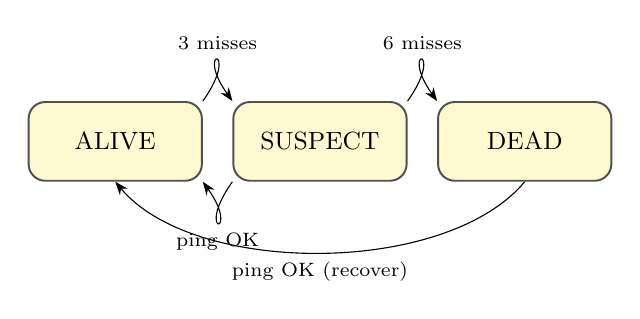
\begin{tikzpicture}[node distance=2.6cm, on grid, >=Stealth,
  st/.style={draw=bordercolor, line width=0.7pt, rounded corners=6pt,
             fill=svcyellow, minimum width=2.2cm, minimum height=1cm,
             font=\small, align=center}]
  \node[st] (a) {ALIVE};
  \node[st, right=of a] (s) {SUSPECT};
  \node[st, right=of s] (d) {DEAD};

  \draw[-{Stealth}] (a.north east) .. controls +(0.5,0.7) and +(-0.5,0.7) ..
        node[above, font=\scriptsize]{3 misses} (s.north west);
  \draw[-{Stealth}] (s.north east) .. controls +(0.5,0.7) and +(-0.5,0.7) ..
        node[above, font=\scriptsize]{6 misses} (d.north west);
  \draw[-{Stealth}] (s.south west) .. controls +(-0.5,-0.7) and +(0.5,-0.7) ..
        node[below, font=\scriptsize]{ping OK} (a.south east);
  \draw[-{Stealth}] (d.south) .. controls +(-1,-1.2) and +(1,-1.2) ..
        node[below, font=\scriptsize]{ping OK (recover)} (a.south);
\end{tikzpicture}
\caption{Peer health state machine. Counters reset on any successful
ping; the \texttt{SUSPECT} and \texttt{DEAD} transitions are hard-coded
to missed-ping thresholds rather than a $\phi$-accrual estimator.}
\label{fig:health-sm}
\end{figure}
 
\subsubsection{Consensus on Group Membership}

Each node maintains a peer registry (added via \texttt{POST /admin/peers/register}). The group is considered healthy when $>$50\% of registered peers are ALIVE; below this threshold the node enters \texttt{LOCAL\_ONLY} mode. This is a lightweight threshold quorum — sufficient for a two-laptop demo without full Paxos/Raft complexity.

\subsubsection{Partition Tolerance}

\texttt{shared/partition.py} probes Postgres, RabbitMQ, and the Conflict Service every 5\,s, cycling through \textbf{CONNECTED} $\to$ \textbf{SUSPECTED} $\to$ \textbf{PARTITIONED} $\to$ \textbf{MERGING}. The current state is attached to every HTTP response as \texttt{X-Partition-Status}. During PARTITIONED, the Enforcement Service continues from cache and adds \texttt{X-Cache-Stale: true}. The state is exposed at /health/partitions.

\subsubsection{Cross-Node Slot Replication}
\label{sec:replication}

The multi-node deployment replicates conflict-service slot state across laptops so a booking on Node A conflicts with one on Node B for the same road segment. Three mechanisms: (1) \textbf{forward push} — after each successful \texttt{checkConflicts()} commit, a goroutine asynchronously sends \texttt{POST /internal/slots/replicate} to every peer; (2) \textbf{catch-up sync} — on boot, each node fetches \texttt{GET /internal/slots/active} from all peers and applies missing rows; (3) \textbf{5-minute periodic re-sync} — a background goroutine repeats the catch-up as a safety net. All writes use \texttt{applyReplicatedSlot}, which is idempotent (keyed by \texttt{journey\_id}). This is deliberately eventually-consistent: two bookings submitted simultaneously to two nodes within the replication window can both pass. This is documented as a known trade-off (Section~\ref{sec:testing}).

\subsubsection{Consistent-Hash Sharding}

Both User Service and Conflict Service assign write authority via MD5 hash: \texttt{shard = MD5(key) \% num\_nodes} where key is the email (users) or route ID (routes). The node where \texttt{shard == 0} is PRIMARY. \emph{All nodes store all data} (active-active replication) — sharding governs write authority only, so reads can be served from any node (locality). Shard role is logged on every operation and surfaced in the activity feed.

\subsubsection{Client-Side Failover}

Every browser API call goes through \texttt{resilientFetch}, which tries the primary URL first, then each peer in the ALIVE list on \texttt{5xx} or network error (\texttt{4xx} passes through unchanged — a rejected booking is not a node failure). The peer list is fetched from \texttt{/health/nodes} at login and persisted to \texttt{localStorage}, enabling failover even before authentication. The WebSocket to \texttt{/ws/notifications/} uses the same list, cycling to a peer after two consecutive disconnects.

% ============================================================
% 6. TESTING
% ============================================================
\section{Testing}
\label{sec:testing}
 
\subsection{Test Plan}

Testing was conducted at three levels: (1) \textbf{Automated end-to-end} — \texttt{scripts/demo\_local.py} runs 11 steps covering health, registration, saga booking, 2PC, conflict detection, cancellation, notifications, enforcement, analytics, outbox durability, and circuit breaker; (2) \textbf{Interactive simulation} — \texttt{scripts/simulate\_problems.py} provides 7 CLI scenarios (data conflict, concurrent storm, 2PC demo, failure detection, circuit breaker, graceful degradation, outbox); (3) \textbf{Multi-device} — two laptops on a shared hotspot, registering each other as peers, documented in \texttt{docs/MULTI\_LAPTOP\_DEMO.md}.
 
\subsection{Test Results}

Table~\ref{tab:results} shows the post-fix end-to-end matrix (slim stack, M1 MacBook). \emph{partial} = works in demo with caveats; \emph{miss} = documented gap.

\begin{table}[H]
\centering\footnotesize
\begin{tabularx}{\textwidth}{L{4.8cm} L{1.2cm} X}
  \toprule
  \textbf{Capability} & \textbf{Status} & \textbf{Evidence / caveat} \\
  \midrule
  User register / login / vehicle register & PASS & \texttt{demo\_local.py} steps 1--3 \\
  JWT authentication cross-node            & PASS & Laptop A token accepted on Laptop B \\
  Booking saga (single node)               & PASS & \texttt{CONFIRMED} within ${\approx}250$\,ms p95 \\
  Idempotent retries                       & PASS & Same \texttt{Idempotency-Key} returns cached journey \\
  Conflict detection (single node)         & PASS & Second booking of same slot \texttt{REJECTED} \\
  Conflict detection (cross-node)          & PASS & Replication lag ${<}200$\,ms on LAN \\
  Two-phase commit booking                 & PASS & \texttt{?mode=2pc} commits atomically \\
  Concurrent booking storm (10 parallel)   & PASS & Exactly 1 \texttt{CONFIRMED}, 9 \texttt{REJECTED} \\
  Circuit breaker                          & PASS & Opens after 3 failures; closes after probe \\
  Transactional outbox survives RabbitMQ restart & PASS & Event drains on reconnect \\
  Enforcement verification (cache hit)     & PASS & Returns \texttt{is\_valid=true} under 10\,ms \\
  Enforcement verification (cache miss)    & PASS & Fallback REST path under 100\,ms \\
  Postgres streaming replication           & PASS & Lag visible at \texttt{/api/analytics/replica-lag} \\
  Redis Sentinel failover                  & PASS & Service reconnects automatically \\
  Node failure detection ALIVE$\to$SUSPECT$\to$DEAD & PASS & Thresholds 3 / 6 missed pings \\
  Client-side failover (login \& all ops)  & PASS & Topbar switches to \texttt{Failover: <ip>} \\
  WebSocket failover                       & PASS & Reconnects to peer after 2 closes \\
  Cascade kill (journey + user 503)        & PASS & \texttt{/admin/simulate/fail} + cascade \\
  Conflict-service peer failover           & PASS & Local conflict-service stopped; booking routed to peer conflict-service via \texttt{conflict\_client.py} \\
  Partition detection state machine        & partial & Correct on dependency loss; not demoed on a live WAN partition \\
  RabbitMQ 3-node cluster                  & partial & Single node stable; cluster joining unreliable on one host \\
  Saga compensation on conflict failure    & miss    & Booking fails fast; no automatic retry \\
  Distributed tracing (spans)              & miss    & Correlation IDs propagate; no Jaeger view \\
  \bottomrule
\end{tabularx}
\caption{End-to-end test results}
\label{tab:results}
\end{table}

All 7 simulation scenarios produced expected outcomes. Notable bugs found during testing (full log in \texttt{docs/DEBUGGING\_LOG.md}): (1) \emph{schema drift} — \texttt{journeys.route\_id} missing in live DB, crashing lifecycle scheduler; fixed with \texttt{ALTER TABLE}; (2) \emph{Docker Compose override silently ignored} — \texttt{DATABASE\_READ\_URL: ""} does not clear the base value, causing reads to fail with \texttt{gaierror}; fixed by setting it explicitly; (3) \emph{nginx stale upstream IP} — after container recreation, nginx cached old IP returning 404; fixed by switching to per-request DNS resolution (\texttt{set \$svc}); (4) \emph{silent cross-node isolation} — two laptops with separate Postgres produced no conflicts, driving the replication design.

\textbf{Known limitation:} Without a consensus protocol, two bookings submitted simultaneously to two nodes can both pass within the replication window. This is an accepted trade-off of active-active eventual consistency; peak booking rates are well below the millisecond boundary in the demo load.

\section{Allocation of Work}
\label{sec:allocation}

\begin{table}[H]
    \centering\small
    \begin{tabularx}{\textwidth}{L{3.2cm} X}
        \toprule
        \textbf{Member} & \textbf{Primary responsibilities} \\
        \midrule
        Parth Deshmukh & User Service: JWT, bcrypt, read/write separation, distributed lock, active-active replication, cascade-kill middleware; Postgres replication setup. \\
        Tanmay Ghosh & Journey Service: booking saga, transactional outbox, circuit breaker, idempotency, lifecycle scheduler, 2PC coordinator, peer health monitor, \texttt{conflict\_client.py}; frontend, docker-compose, shared Python modules. \\
        Sneha Meto & Conflict Service: grid-cell model, \texttt{SERIALIZABLE} check, cancellation consumer, cross-node slot replication; load-testing scripts. \\
        Aditya Kumar Singh & Notification Service: WebSocket hub, Redis history, exactly-once dedup, DLQ; dashboard live feed. \\
        Saurabh Deshmukh & Enforcement Service: Redis-first lookup, licence cache, event-driven invalidation, stale header; \texttt{MULTI\_LAPTOP\_DEMO.md}. \\
        Sai Eeshwar Divaakar & Analytics Service: dual-write counters, hourly rollup, replica-lag, service health; Redis Sentinel; \texttt{REQUIREMENTS.md}. \\
        \bottomrule
    \end{tabularx}
    \caption{Allocation of work among team members.}
    \label{tab:work-allocation}
\end{table}
 
% ============================================================
% 8. CONCLUSION
% ============================================================
\section{Summary}
\label{sec:conclusion}

The system delivers a globally-accessible, fault-tolerant Journey Booking System across six microservices demonstrating: database-per-service decomposition, synchronous REST sagas + asynchronous RabbitMQ fan-out, transactional outbox (at-least-once delivery), per-endpoint circuit breakers, partition detection, \texttt{SERIALIZABLE}+\texttt{SELECT FOR UPDATE} for strong consistency, PostgreSQL WAL replication (read/write separation), Redis Sentinel (cache HA), TTL-based cache replacement, nginx rate limiting, DLQ routing, idempotent consumers, consistent-hash sharding, Redlock-style 2-phase distributed lock, service-level conflict-service failover (\texttt{conflict\_client.py}), and active-active cross-node slot replication with client-side failover.

Tested on single-laptop slim stack and two-laptop hotspot setup; full-node kill on Laptop A leaves sessions active on Laptop B without re-login. Known trade-offs (documented, not hidden): no consensus protocol (millisecond-window double-booking possible), no saga compensation retry, RabbitMQ cluster unreliable on single host, correlation IDs only (no Jaeger). The system meets all latency and availability targets in Section~\ref{sec:nfr} and passes the full test matrix in Table~\ref{tab:results}.

% ============================================================
% SIGNATURES
% ============================================================
\newpage
\section*{Declaration}
We, the undersigned, confirm that this report accurately represents the work carried out by our Group J for CS7NS6 Exercise~2.

\vspace{1.5cm}

\noindent
\begin{tabular}{p{6cm} p{6cm}}
    \includegraphics[width=3cm,height=1.5cm]{sign/sign_parth.jpeg} & \includegraphics[width=4cm,height=2cm]{sign/sheesh.png} \\
    \rule{5cm}{0.4pt} & \rule{5cm}{0.5pt} \\
    Parth Deshmukh & Sai Eeshwar Divaakar \\[1.5cm]
    \includegraphics[width=4cm,height=2cm]{sign/aditya.png} & \includegraphics[width=4cm,height=2cm]{sign/Tanmay.png} \\
    \rule{5cm}{0.4pt} & \rule{5cm}{0.4pt} \\
    Aditya Kumar Singh & Tanmay Ghosh \\[1.5cm]
    \includegraphics[width=4cm,height=2cm]{sign/Signature_Saurabh.jpeg} & \includegraphics[width=4cm,height=2cm]{sign/sneha.png} \\
    \rule{5cm}{0.4pt} & \rule{5cm}{0.4pt} \\
    Saurabh Deshmukh & Sneha Meto \\
\end{tabular}

\end{document}